\documentclass[preprint,12pt,aps,pra,showkeys,amsmath,amssymb,superscriptaddress,floatfix]{revtex4-2}
\usepackage[T1]{fontenc}
\usepackage[utf8]{inputenc}
\usepackage{amsmath,amssymb,amsthm,mathtools,mathrsfs}
\usepackage{microtype,booktabs,enumitem}
\usepackage{xcolor,tikz,etoolbox}
\usepackage[skins,breakable]{tcolorbox}
\usepackage{needspace}
% Keep diagram geometry independent of REVTeX preprint body spacing.
\AtBeginEnvironment{tikzpicture}{\linespread{1}\selectfont}
\usetikzlibrary{arrows.meta,positioning,calc,fit,decorations.pathreplacing}
\usepackage{graphicx}
\usepackage{hyperref}

\definecolor{MMBlue}{RGB}{0,82,155}
\definecolor{MMOrange}{RGB}{200,80,0}
\tikzset{
 mmnode/.style={draw=MMBlue,rounded corners=2pt,fill=MMBlue!4,align=left,execute at begin node={\raggedright},text width=5cm,font=\fontsize{10}{12}\selectfont,inner sep=6pt},
 mmimport/.style={mmnode,draw=black!65,fill=black!4},
 mmcandidate/.style={mmnode,draw=MMOrange,dashed,fill=MMOrange!5},
 mmrejected/.style={mmnode,draw=black,densely dotted,fill=black!8},
 mmproof/.style={->,thick,MMBlue},
 mmflow/.style={->,semithick,black!70},
 mmrepair/.style={->,dashed,thick,MMOrange},
 mmcandidatearrow/.style={->,dashed,semithick,MMOrange},
 mmnote/.style={font=\scriptsize,fill=white,inner sep=2pt,align=center}}

\usepackage[section]{placeins}
\setlength{\emergencystretch}{3em}
\setlist{itemsep=3pt,topsep=4pt}
\newtheorem{theorem}{Theorem}[section]
\newtheorem{proposition}[theorem]{Proposition}
\newtheorem{lemma}[theorem]{Lemma}
\newtheorem{corollary}[theorem]{Corollary}
\theoremstyle{definition}
\newtheorem{definition}[theorem]{Definition}
\newtheorem{example}[theorem]{Example}
\theoremstyle{remark}
\newtheorem{remark}[theorem]{Remark}
% Avoid isolated statement headings and single-line paragraph fragments.
\BeforeBeginEnvironment{theorem}{\Needspace{6\baselineskip}}
\BeforeBeginEnvironment{definition}{\Needspace{5\baselineskip}}
\BeforeBeginEnvironment{proposition}{\Needspace{5\baselineskip}}
\BeforeBeginEnvironment{lemma}{\Needspace{5\baselineskip}}
\BeforeBeginEnvironment{corollary}{\Needspace{5\baselineskip}}
\clubpenalty=5000
\widowpenalty=5000
\newcommand{\R}{\mathbb R}\newcommand{\Z}{\mathbb Z}\newcommand{\N}{\mathbb N}
\newcommand{\Pa}{\operatorname{Pa}}\newcommand{\Desc}{\operatorname{Desc}}
\newcommand{\cl}{\operatorname{cl}}\newcommand{\cost}{\operatorname{cost}}
\newcommand{\status}{\operatorname{status}}
% Faculty cards: a visual rail groups the five faculties within one agent.
% The rail has no arrowhead and does not represent a proof dependency.
\newcommand{\mmfacultybadge}[1]{%
 \node[circle,draw=MMBlue,line width=1pt,fill=white,
 minimum size=7mm,inner sep=0pt,font=\sffamily\small\bfseries,text=MMBlue]
 at ([xshift=15pt,yshift=-15pt]frame.north west) {#1};}
\newcommand{\mmfacultyrail}{%
 \draw[MMBlue!80,line width=1pt]
 ([xshift=15pt,yshift=2pt]frame.north west)--
 ([xshift=15pt,yshift=-2pt]frame.south west);}
\newtcolorbox{mmfacultybox}[2]{enhanced,breakable,
 colback=MMBlue!4,colframe=MMBlue!4,boxrule=0pt,arc=3pt,
 left=39pt,right=9pt,top=4pt,bottom=4pt,
 before skip=2pt,after skip=2pt,
 fontupper=\small\linespread{1.1}\selectfont,
 overlay unbroken={\mmfacultyrail\mmfacultybadge{#1}},
 overlay first={\mmfacultyrail\mmfacultybadge{#1}},
 overlay middle={\mmfacultyrail},overlay last={\mmfacultyrail}}
\newcommand{\mmfaculty}[3]{%
 \begin{mmfacultybox}{#1}{#2}
 {\sffamily\bfseries\color{MMBlue}#2}\par\smallskip #3
 \end{mmfacultybox}}
\newcommand{\agent}[9]{%
 \Needspace{8\baselineskip}
 \subsubsection{#1}
 \noindent\textbf{Object.} #2\par
 \noindent\textbf{Role.} #3\par\smallskip
 \mmfaculty{E}{Ego}{#4}
 \mmfaculty{M}{Memory}{#5}
 \mmfaculty{I}{Intellect}{#6}
 \mmfaculty{S}{Sense}{#7}
 \mmfaculty{A}{Action}{#8}
 \smallskip\noindent #9\par}

\usepackage{longtable,array,calc}
\providecommand{\tightlist}{\setlength{\itemsep}{2pt}\setlength{\parskip}{0pt}}
\makeatletter
\def\frontmatter@abstract@produce{\par\addvspace{\frontmatter@preabstractspace}%
\begingroup\prep@absbox\unvbox\absbox\post@absbox\endgroup
\addvspace{\frontmatter@postabstractspace}}
\makeatother
\newcommand{\field}[2]{\par\smallskip\noindent\textbf{#1.} #2\par}
\setlength{\emergencystretch}{5em}
\AtBeginEnvironment{verbatim}{\small\linespread{1.0}\selectfont}


\hypersetup{colorlinks=true,linkcolor=MMBlue,urlcolor=MMBlue,pdfauthor={Dibakar Sigdel}}

\begin{document}

\title{Riemann Mapping Theorem\\[4pt]\large An End-to-End Meta-Math Walkthrough}

\author{Dibakar Sigdel}

\affiliation{Mindverse Computing LLC, Lynnwood, WA 98087, USA}

\date{October 2026}

\begin{abstract}

A complete authored walkthrough of riemann mapping theorem, with
explicit mathematical contracts, local verification gates, and reusable
exports. The report presents the target theorem, declared imports, a
dependency graph, five-faculty node contracts, a continuous proof, a
worked example, and a hypothesis-repair audit. It is an authored
mathematical exposition, not a deployed-agent transcript or a formal
proof-assistant certificate.

\end{abstract}\maketitle\linespread{1.12}\selectfont

\noindent\textbf{CA-05 / Complex Analysis / Report v1}

\section{Target and import contract}

\begin{theorem}

For a nonempty simply connected proper domain
\(\Omega\subsetneq\mathbb C\) and \(z_0\in\Omega\), prove there is a
unique biholomorphism \(F:\Omega\to\mathbb D\) with \(F(z_0)=0\) and
\(F'(z_0)>0\) real.

\end{theorem}

\subsection{Foundations and permitted imports}

Use these imported complex-analytic modules: on a simply connected
domain every nowhere-zero holomorphic function has a holomorphic
logarithm and hence a square root; a locally bounded holomorphic family
has a locally uniformly convergent subsequence (Montel); a locally
uniform limit of injective holomorphic functions is injective or
constant (Hurwitz consequence); the maximum modulus principle; Schwarz's
lemma; Cauchy's derivative bound; disk automorphisms
\(\varphi _b(w)=(w-b)/(1-\operatorname{conj} (b)w)\). These supporting
results are substantial and are not proved here. The target mapping
theorem is not imported.

Also use the open mapping theorem and the local inverse theorem for a
holomorphic injective map (its derivative is nonzero). These supporting
complex-analysis modules are declared imports.

\clearpage\section{Node interaction workflow}

\begin{center}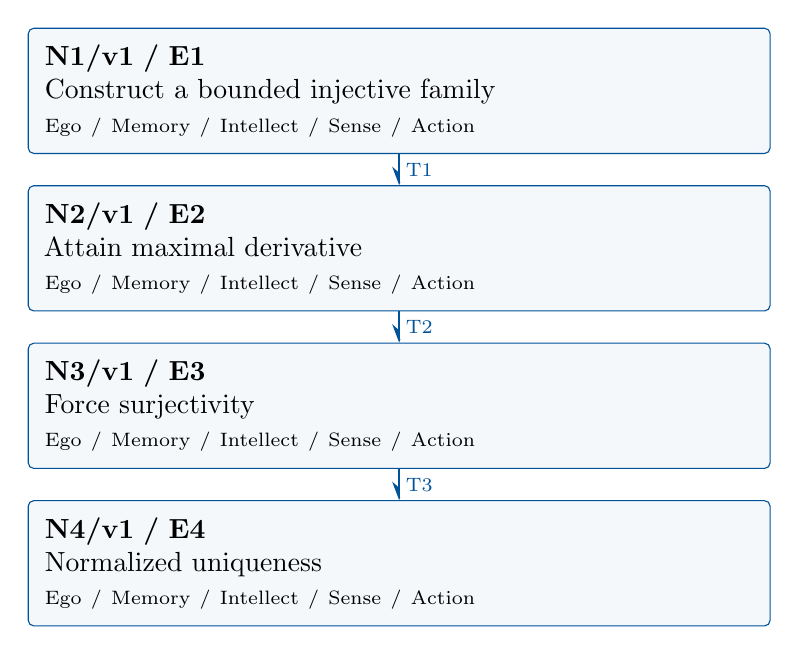
\begin{tikzpicture}[>=Stealth,x=1cm,y=1cm]

\node[mmnode,text width=9cm,minimum height=1.25cm] (N1) at (0,0.0) {\textbf{N1/v1 / E1}\\Construct a bounded injective family\\{\scriptsize Ego / Memory / Intellect / Sense / Action}};

\node[mmnode,text width=9cm,minimum height=1.25cm] (N2) at (0,-2.0) {\textbf{N2/v1 / E2}\\Attain maximal derivative\\{\scriptsize Ego / Memory / Intellect / Sense / Action}};

\node[mmnode,text width=9cm,minimum height=1.25cm] (N3) at (0,-4.0) {\textbf{N3/v1 / E3}\\Force surjectivity\\{\scriptsize Ego / Memory / Intellect / Sense / Action}};

\node[mmnode,text width=9cm,minimum height=1.25cm] (N4) at (0,-6.0) {\textbf{N4/v1 / E4}\\Normalized uniqueness\\{\scriptsize Ego / Memory / Intellect / Sense / Action}};

\draw[mmproof] (N1.south) -- node[mmnote,right] {T1} (N2.north);

\draw[mmproof] (N2.south) -- node[mmnote,right] {T2} (N3.north);

\draw[mmproof] (N3.south) -- node[mmnote,right] {T3} (N4.north);

\end{tikzpicture}\end{center}

Each box is one mathematical agent containing all five faculties. Blue
arrows carry the versioned exports listed below. The layout gives a
reading order; only drawn arrows assert dependencies. Diagnostic repair
is separate from the proof DAG.

\clearpage\subsection{Versioned evidence-transfer ledger}

\begingroup\small\linespread{1.05}\selectfont

\Needspace{5\baselineskip}\field{T1: N1/E1/v1 to N2}{The family of injective maps \(\Omega \to D\) with value 0 and positive
derivative at \(z_{0}\) is nonempty.}

\field{Receiving activity}{N2: Attain maximal derivative}

\field{Compatibility}{Use the same mathematical objects and hypotheses as the source export.
Receiving contract: Normalized family; Montel and Cauchy bounds; prior
exports E1/v1}

\Needspace{5\baselineskip}\field{T2: N2/E2/v1 to N3}{An injective normalized extremizer F with \(F'(z_{0})=\alpha >0\).}

\field{Receiving activity}{N3: Force surjectivity}

\field{Compatibility}{Use the same mathematical objects and hypotheses as the source export.
Receiving contract: Extremizer F; hypothetical omitted \(b\in D\); prior
exports E2/v1}

\Needspace{5\baselineskip}\field{T3: N3/E3/v1 to N4}{F is a biholomorphism \(\Omega \to D\).}

\field{Receiving activity}{N4: Normalized uniqueness}

\field{Compatibility}{Use the same mathematical objects and hypotheses as the source export.
Receiving contract: Two biholomorphisms with the same normalization;
prior exports E3/v1}

\endgroup

\clearpage\section{Agent roles and five-faculty activities}\begingroup\small\linespread{1.05}\selectfont\setlist{itemsep=1pt,topsep=2pt}

\subsection{N1/v1: Construct a bounded injective family}

\field{Object and role}{Take a square root, omit an open disk, then reciprocate.}

\field{Inputs}{Proper simply connected \(\Omega\) and \(z_{0}\); foundational imports
stated in §1}

\mmfaculty{E}{Ego}{Own E1/v1: The family of injective maps \(\Omega \to D\) with value 0
and positive derivative at \(z_{0}\) is nonempty.}

\mmfaculty{M}{Memory}{Retain Proper simply connected \(\Omega\) and \(z_{0}\); foundational
imports stated in §1; keep their assumptions and versions attached.}

\mmfaculty{I}{Intellect}{Take a square root, omit an open disk, then reciprocate.}

\mmfaculty{S}{Sense}{Properness supplies a; a branch must be global on \(\Omega\).}

\mmfaculty{A}{Action}{Carry out the numbered deductions and publish E1/v1 together with its
hypotheses and proof location.}

\smallskip\noindent\textbf{Numbered mathematical activities}

\begin{enumerate}[label=N1.\arabic*,leftmargin=3.4em]

\item Choose \(a\notin \Omega\) and a branch \(h(z)=\sqrt{z-a}\).

\item It is injective since equality of h implies equality after squaring.

\item Its image is disjoint from its negative: \(h(z_{1})=-h(z_{2})\) would
give \(z_{1}=z_{2}\) and \(h(z_{1})=0\), impossible.

\item Let \(w_{0}=h(z_{0})\); the open image contains \(B(w_{0},r)\) for some
\(r>0\), so it omits \(B(-w_{0},r)\).

\item Thus \(q(z)=1/(h(z)+w_{0})\) is injective, holomorphic, and bounded by
1/r.

\item Scale it strictly into D, apply a disk automorphism to make the value at
\(z_{0}\) zero, and rotate so its nonzero derivative is positive real.

\item This gives a nonempty family F of normalized injective maps
\(\Omega \to D\).

\end{enumerate}

\field{Export E1/v1}{The family of injective maps \(\Omega \to D\) with value 0 and positive
derivative at \(z_{0}\) is nonempty.}

\field{Acceptance gate}{Properness supplies a; a branch must be global on \(\Omega\). Publish
only after checking every displayed deduction.}

\field{Targeted repair}{If the check fails, revise N1: Properness supplies a; a branch must be
global on \(\Omega\). Recheck dependent nodes N2, N3, N4.}

\clearpage

\subsection{N2/v1: Attain maximal derivative}

\field{Object and role}{Take an extremal sequence with a nonconstant limit.}

\field{Inputs}{Normalized family; Montel and Cauchy bounds; prior exports E1/v1}

\mmfaculty{E}{Ego}{Own E2/v1: An injective normalized extremizer F with
\(F'(z_{0})=\alpha >0\).}

\mmfaculty{M}{Memory}{Retain Normalized family; Montel and Cauchy bounds; prior exports E1/v1;
keep their assumptions and versions attached.}

\mmfaculty{I}{Intellect}{Take an extremal sequence with a nonconstant limit.}

\mmfaculty{S}{Sense}{A constant limit must be ruled out before invoking injective-limit
preservation.}

\mmfaculty{A}{Action}{Carry out the numbered deductions and publish E2/v1 together with its
hypotheses and proof location.}

\smallskip\noindent\textbf{Numbered mathematical activities}

\begin{enumerate}[label=N2.\arabic*,leftmargin=3.4em]

\item Choose a closed disk about \(z_{0}\) contained in \(\Omega\).

\item Cauchy's estimate bounds every family derivative at \(z_{0}\) by one
common finite constant.

\item Let \(\alpha\) be the supremum of the positive derivatives; it is
positive by nonemptiness.

\item Pick \(f_j\) with \(f_j'(z_{0})\to \alpha\).

\item Montel provides a locally uniform limit F, with \(F(z_{0})=0\) and
\(F'(z_{0})=\alpha\) by Cauchy's formula.

\item It is nonconstant.

\item Hurwitz makes F injective, and the maximum modulus principle upgrades
\(|F|\le 1\) to \(|F|<1\).

\item Thus F belongs to the family and attains \(\alpha\).

\end{enumerate}

\field{Export E2/v1}{An injective normalized extremizer F with \(F'(z_{0})=\alpha >0\).}

\field{Acceptance gate}{A constant limit must be ruled out before invoking injective-limit
preservation. Publish only after checking every displayed deduction.}

\field{Targeted repair}{If the check fails, revise N2: A constant limit must be ruled out before
invoking injective-limit preservation. Recheck dependent nodes N3, N4.}

\clearpage

\subsection{N3/v1: Force surjectivity}

\field{Object and role}{Construct a normalized map with a larger derivative.}

\field{Inputs}{Extremizer F; hypothetical omitted \(b\in D\); prior exports E2/v1}

\mmfaculty{E}{Ego}{Own E3/v1: F is a biholomorphism \(\Omega \to D\).}

\mmfaculty{M}{Memory}{Retain Extremizer F; hypothetical omitted \(b\in D\); prior exports
E2/v1; keep their assumptions and versions attached.}

\mmfaculty{I}{Intellect}{Construct a normalized map with a larger derivative.}

\mmfaculty{S}{Sense}{The derivative improvement must be strict, not merely nondecreasing.}

\mmfaculty{A}{Action}{Carry out the numbered deductions and publish E3/v1 together with its
hypotheses and proof location.}

\smallskip\noindent\textbf{Numbered mathematical activities}

\begin{enumerate}[label=N3.\arabic*,leftmargin=3.4em]

\item Suppose \(b\in D\setminus F(\Omega )\).

\item Because \(F(z_{0})=0\), \(b\ne 0\).

\item Let \(r=|b|\in (0,1)\) and \(H=\varphi _b\circ F\), which never
vanishes.

\item Take a holomorphic square root h of H on \(\Omega\).

\item Since \(|H|<1\), h maps into D, and it is injective by squaring.

\item Write \(c=h(z_{0})\); then \(|c|=\sqrt{r}\).

\item The normalized map \(\psi _c\circ h\), followed by a rotation, belongs
to the family.

\item Its derivative modulus at \(z_{0}\) is
\(\alpha (1-r^{2})/(2\sqrt{r(1}-r))=\alpha (1+r)/(2\sqrt{r)>\alpha }\)
because \((1-\sqrt{r)^{2}>0}\).

\item This contradicts maximality.

\item Hence F is onto D.

\item Its derivative never vanishes by holomorphic injectivity, and the local
inverse theorem gives a holomorphic inverse.

\end{enumerate}

\field{Export E3/v1}{F is a biholomorphism \(\Omega \to D\).}

\field{Acceptance gate}{The derivative improvement must be strict, not merely nondecreasing.
Publish only after checking every displayed deduction.}

\field{Targeted repair}{If the check fails, revise N3: The derivative improvement must be
strict, not merely nondecreasing. Recheck dependent nodes N4.}

\clearpage

\subsection{N4/v1: Normalized uniqueness}

\field{Object and role}{Apply Schwarz to the transition map and its inverse.}

\field{Inputs}{Two biholomorphisms with the same normalization; prior exports E3/v1}

\mmfaculty{E}{Ego}{Own E4/v1: Existence and uniqueness of the specified normalized
biholomorphism.}

\mmfaculty{M}{Memory}{Retain Two biholomorphisms with the same normalization; prior exports
E3/v1; keep their assumptions and versions attached.}

\mmfaculty{I}{Intellect}{Apply Schwarz to the transition map and its inverse.}

\mmfaculty{S}{Sense}{Dropping the positive-derivative condition leaves rotational freedom.}

\mmfaculty{A}{Action}{Carry out the numbered deductions and publish E4/v1 together with its
hypotheses and proof location.}

\smallskip\noindent\textbf{Numbered mathematical activities}

\begin{enumerate}[label=N4.\arabic*,leftmargin=3.4em]

\item If F and G are normalized, \(A=G\circ F^{-1}\) is an automorphism of D
fixing 0.

\item Schwarz applied to A and \(A^{-1}\) gives \(|A'(0)|=1\) and the equality
case \(A(w)=e^{i\theta }w\).

\item But \(A'(0)=G'(z_{0})/F'(z_{0})\) is positive real; hence it equals 1
and A is the identity.

\item Thus \(G=F\).

\end{enumerate}

\field{Export E4/v1}{Existence and uniqueness of the specified normalized biholomorphism.}

\field{Acceptance gate}{Dropping the positive-derivative condition leaves rotational freedom.
Publish only after checking every displayed deduction.}

\field{Targeted repair}{If the check fails, revise N4: Dropping the positive-derivative
condition leaves rotational freedom. Withhold this terminal result until
its gate passes.}

\endgroup\clearpage\section{Continuous mathematical proof}\label{sec:proof}

Read these steps in order as one proof; the diagram is optional.
Numbered activities identify the specific constructions and deductions
owned by each node.

\subsection{§4.N1 --- Construct a bounded injective
family}\label{n1-construct-a-bounded-injective-family}

\begin{enumerate}
\def\labelenumi{\arabic{enumi}.}
\item
  Choose \(a\notin \Omega\) and a branch \(h(z)=\sqrt{z-a}\).
\item
  It is injective since equality of h implies equality after squaring.
\item
  Its image is disjoint from its negative: \(h(z_{1})=-h(z_{2})\) would
  give \(z_{1}=z_{2}\) and \(h(z_{1})=0\), impossible.
\item
  Let \(w_{0}=h(z_{0})\); the open image contains \(B(w_{0},r)\) for
  some \(r>0\), so it omits \(B(-w_{0},r)\).
\item
  Thus \(q(z)=1/(h(z)+w_{0})\) is injective, holomorphic, and bounded by
  1/r.
\item
  Scale it strictly into D, apply a disk automorphism to make the value
  at \(z_{0}\) zero, and rotate so its nonzero derivative is positive
  real.
\item
  This gives a nonempty family F of normalized injective maps
  \(\Omega \to D\).
\end{enumerate}

\subsection{§4.N2 --- Attain maximal
derivative}\label{n2-attain-maximal-derivative}

\begin{enumerate}
\def\labelenumi{\arabic{enumi}.}
\item
  Choose a closed disk about \(z_{0}\) contained in \(\Omega\).
\item
  Cauchy's estimate bounds every family derivative at \(z_{0}\) by one
  common finite constant.
\item
  Let \(\alpha\) be the supremum of the positive derivatives; it is
  positive by nonemptiness.
\item
  Pick \(f_j\) with \(f_j'(z_{0})\to \alpha\).
\item
  Montel provides a locally uniform limit F, with \(F(z_{0})=0\) and
  \(F'(z_{0})=\alpha\) by Cauchy's formula.
\item
  It is nonconstant.
\item
  Hurwitz makes F injective, and the maximum modulus principle upgrades
  \(|F|\le 1\) to \(|F|<1\).
\item
  Thus F belongs to the family and attains \(\alpha\).
\end{enumerate}

\subsection{§4.N3 --- Force surjectivity}\label{n3-force-surjectivity}

\begin{enumerate}
\def\labelenumi{\arabic{enumi}.}
\item
  Suppose \(b\in D\setminus F(\Omega )\).
\item
  Because \(F(z_{0})=0\), \(b\ne 0\).
\item
  Let \(r=|b|\in (0,1)\) and \(H=\varphi _b\circ F\), which never
  vanishes.
\item
  Take a holomorphic square root h of H on \(\Omega\).
\item
  Since \(|H|<1\), h maps into D, and it is injective by squaring.
\item
  Write \(c=h(z_{0})\); then \(|c|=\sqrt{r}\).
\item
  The normalized map \(\psi _c\circ h\), followed by a rotation, belongs
  to the family.
\item
  Its derivative modulus at \(z_{0}\) is
  \(\alpha (1-r^{2})/(2\sqrt{r(1}-r))=\alpha (1+r)/(2\sqrt{r)>\alpha }\)
  because \((1-\sqrt{r)^{2}>0}\).
\item
  This contradicts maximality.
\item
  Hence F is onto D.
\item
  Its derivative never vanishes by holomorphic injectivity, and the
  local inverse theorem gives a holomorphic inverse.
\end{enumerate}

\subsection{§4.N4 --- Normalized
uniqueness}\label{n4-normalized-uniqueness}

\begin{enumerate}
\def\labelenumi{\arabic{enumi}.}
\item
  If F and G are normalized, \(A=G\circ F^{-1}\) is an automorphism of D
  fixing 0.
\item
  Schwarz applied to A and \(A^{-1}\) gives \(|A'(0)|=1\) and the
  equality case \(A(w)=e^{i\theta }w\).
\item
  But \(A'(0)=G'(z_{0})/F'(z_{0})\) is positive real; hence it equals 1
  and A is the identity.
\item
  Thus \(G=F\).
\end{enumerate}

\hfill$\square$

\section{Worked orchestration}

For the upper half-plane \(\Omega\) and \(z_{0}=i\),
\(F(z)=i(z-i)/(z+i)\) maps \(\Omega\) onto D. The Cayley transform has
unit-circle boundary values and maps i to 0; multiplication by i rotates
the disk. Direct differentiation gives \(F'(i)=1/2>0\), matching the
normalization.

\subsection{Boundary and hypothesis audit}

A multiply connected annulus cannot be biholomorphic to D because
biholomorphisms preserve fundamental groups. For \(\Omega =C\), a map
into D would be bounded entire and constant by Liouville. Sense checks
these domain exclusions before attempting the square-root/extremal
proof.

\section{Illustrative failure and repair}

The following is an authored diagnostic scenario. Changed assumptions
define a new contract; they do not retroactively prove the original
statement.

\subsection{Failure and correction}
This is an authored teaching trace, not a recorded agent run.

\begin{enumerate}
\def\labelenumi{\arabic{enumi}.}
\tightlist
\item
  \textbf{Ego \(\to\) Memory:} register the §1 theorem, imports, and
  requested exports before beginning the proof.
\item
  \textbf{Intellect \(\to\) Action:} choose the bridges in §3 and carry
  out the numbered activities in §4; transmit only established E-exports
  along the §2 DAG.
\item
  \textbf{Sense \(\to\) responsible node:} test the specific
  boundary/failure in §5 and the node's individual audit. A failing
  candidate is withheld; downstream nodes may not use it.
\item
  \textbf{Memory + Intellect:} identify whether the error is an omitted
  condition, an invalid inference, or an attempted extension beyond the
  theorem. Restore the exact contract or explicitly state a different
  one.
\item
  \textbf{Action:} redo the affected mathematical activity using the
  repaired condition or inference. Recheck consuming nodes, rather than
  feeding their conclusions back as premises.
\item
  \textbf{Ego:} publish only the supported export with its assumptions
  and proof location. A hypothetical revised export is v2; the written
  proof here is the v1 exposition, not a claim that this repair was
  executed.
\end{enumerate}

\subsection{Hypothesis boundary}
A multiply connected annulus cannot be biholomorphic to D because
biholomorphisms preserve fundamental groups. For \(\Omega =C\), a map
into D would be bounded entire and constant by Liouville. Sense checks
these domain exclusions before attempting the square-root/extremal
proof.

\subsection{Version and recheck}
Version changed contracts and recheck the revised export and every
dependent node. Diagnostic feedback is not a proof premise.

\par\medskip\begingroup\footnotesize\linespread{1.0}\selectfont\noindent\textbf{Provenance.} This authored proof is complete relative to its declared imports. Reuse
each export with its assumptions, proof, and version. The original
Markdown remains available for comparison.
\par\endgroup

\par\smallskip\begingroup\footnotesize\linespread{1.0}\selectfont\noindent\textbf{Further reading.} \begin{itemize}
\item
  \href{https://people.math.harvard.edu/~siu/math113/}{Harvard complex
  analysis: Cauchy formula, argument principle, and Riemann mapping
  lectures}.
\item
  \href{https://people.math.harvard.edu/~siu/math113/15_riemann_mapping_theorem.pdf}{Harvard
  Riemann Mapping Theorem lecture}.
\end{itemize}\par\endgroup

\end{document}
